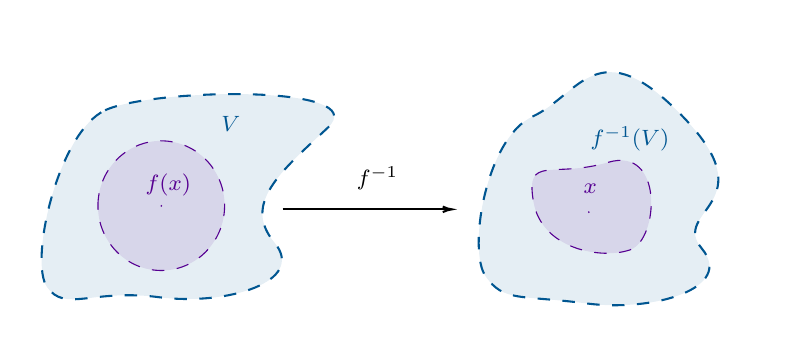
\begin{tikzpicture}[x=0.75pt,y=0.75pt,yscale=-1,xscale=1]
	%uncomment if require: \path (0,300); %set diagram left start at 0, and has height of 300

	%Shape: Polygon Curved [id:ds9863252903529107] 
	\draw  [color={rgb, 255:red, 0; green, 86; blue, 145 }  ,draw opacity=1 ][fill={rgb, 255:red, 0; green, 86; blue, 145 }  ,fill opacity=0.1 ][dash pattern={on 4.5pt off 4.5pt}][line width=0.75]  (57.97,33.79) .. controls (80.65,23.22) and (187.88,21.11) .. (165.2,42.24) .. controls (142.52,63.36) and (123.85,78.74) .. (139.52,97.54) .. controls (155.2,116.35) and (116.63,128.1) .. (84,123.88) .. controls (51.37,119.65) and (38.86,131.38) .. (30,119) .. controls (21.14,106.62) and (35.29,44.35) .. (57.97,33.79) -- cycle ;
	%Shape: Ellipse [id:dp7045194170512884] 
	\draw  [color={rgb, 255:red, 86; green, 0; blue, 145 }  ,draw opacity=1 ][fill={rgb, 255:red, 86; green, 0; blue, 145 }  ,fill opacity=0.1 ][dash pattern={on 4.5pt off 4.5pt}] (54.5,79.77) .. controls (54.5,62.52) and (68.16,48.54) .. (85.01,48.54) .. controls (101.86,48.54) and (115.52,62.52) .. (115.52,79.77) .. controls (115.52,97.02) and (101.86,111) .. (85.01,111) .. controls (68.16,111) and (54.5,97.02) .. (54.5,79.77) -- cycle ;
	%Shape: Ellipse [id:dp17380935073260606] 
	\draw  [color={rgb, 255:red, 86; green, 0; blue, 145 }  ,draw opacity=1 ][dash pattern={on 4.5pt off 4.5pt}] (84.91,79.87) .. controls (84.91,79.82) and (84.96,79.77) .. (85.01,79.77) .. controls (85.07,79.77) and (85.11,79.82) .. (85.11,79.87) .. controls (85.11,79.93) and (85.07,79.98) .. (85.01,79.98) .. controls (84.96,79.98) and (84.91,79.93) .. (84.91,79.87) -- cycle ;

	%Straight Lines [id:da5395275905863334] 
	\draw [line width=0.75]    (143.52,81.54) -- (223,81.54) ;
	\draw [shift={(225,81.54)}, rotate = 180] [color={rgb, 255:red, 0; green, 0; blue, 0 }  ][line width=0.75]    (4.37,-1.32) .. controls (2.78,-0.56) and (1.32,-0.12) .. (0,0) .. controls (1.32,0.12) and (2.78,0.56) .. (4.37,1.32)   ;
	%Shape: Polygon Curved [id:ds45640730182556577] 
	\draw  [color={rgb, 255:red, 0; green, 86; blue, 145 }  ,draw opacity=1 ][fill={rgb, 255:red, 0; green, 86; blue, 145 }  ,fill opacity=0.1 ][dash pattern={on 4.5pt off 4.5pt}][line width=0.75]  (263.97,36.79) .. controls (286.65,26.22) and (295.46,-5.49) .. (336.33,36.88) .. controls (377.2,79.24) and (329.85,81.74) .. (345.52,100.54) .. controls (361.2,119.35) and (322.63,131.1) .. (290,126.88) .. controls (257.37,122.65) and (250.2,126.26) .. (241.33,113.88) .. controls (232.47,101.49) and (241.29,47.35) .. (263.97,36.79) -- cycle ;
	%Shape: Ellipse [id:dp21595437817711993] 
	\draw  [color={rgb, 255:red, 86; green, 0; blue, 145 }  ,draw opacity=1 ][dash pattern={on 4.5pt off 4.5pt}] (290.91,82.87) .. controls (290.91,82.82) and (290.96,82.77) .. (291.01,82.77) .. controls (291.07,82.77) and (291.11,82.82) .. (291.11,82.87) .. controls (291.11,82.93) and (291.07,82.98) .. (291.01,82.98) .. controls (290.96,82.98) and (290.91,82.93) .. (290.91,82.87) -- cycle ;
	%Shape: Polygon Curved [id:ds49186281368908624] 
	\draw  [color={rgb, 255:red, 86; green, 0; blue, 145 }  ,draw opacity=1 ][fill={rgb, 255:red, 86; green, 0; blue, 145 }  ,fill opacity=0.1 ][dash pattern={on 4.5pt off 4.5pt}] (300.33,58.88) .. controls (327.33,50.88) and (324.67,96.13) .. (311,101) .. controls (297.33,105.88) and (268.33,100.88) .. (264.33,77.88) .. controls (260.33,54.88) and (273.33,66.88) .. (300.33,58.88) -- cycle ;

	% Text Node
	\draw (112.65,35.65) node [anchor=north west][inner sep=0.75pt]  [font=\footnotesize,color={rgb, 255:red, 0; green, 86; blue, 145 }  ,opacity=1 ]  {$V$};
	% Text Node
	\draw (76.25,63) node [anchor=north west][inner sep=0.75pt]  [font=\footnotesize,color={rgb, 255:red, 0; green, 145; blue, 105 }  ,opacity=1 ]  {$\textcolor[rgb]{0.34,0,0.57}{f( x)}$};
	% Text Node
	\draw (178,60) node [anchor=north west][inner sep=0.75pt]  [font=\footnotesize]  {$f^{-1}$};
	% Text Node
	\draw (290.65,40.65) node [anchor=north west][inner sep=0.75pt]  [font=\footnotesize,color={rgb, 255:red, 0; green, 86; blue, 145 }  ,opacity=1 ]  {$f^{-1}( V)$};
	% Text Node
	\draw (287.25,68) node [anchor=north west][inner sep=0.75pt]  [font=\footnotesize,color={rgb, 255:red, 86; green, 0; blue, 145 }  ,opacity=1 ]  {$x$};


\end{tikzpicture}
